\lab{Algorithms}{Temporal Complexity and Sparse Matrices}{Complexity and Sparse Matrices}

\objective{Introduce the concept of temporal complexity and explore SciPy's special methods for working with sparse matrices.}

\section*{Temporal Complexity}
One of the most important questions in scientific computing is: how long will this operation take?
The concept of temporal complexity attempts to answer this question by determining how much time a function needs to operate on a given size of input. 
For example, suppose a particular algorithm operating on a matrix of size $n$ (that is, an $n \times n$ matrix) requires the following number of calculations:

\begin{equation*}
f(n) = \frac{3n^3}{2} + 75n^2 + 250n + 30
\end{equation*}

As the input gets larger, the growth of $f(n)$ is dominated by the $n^3$ term.
For this reason we say that $f(n) \in O(n^3)$, or more commonly, that $f(n)$ is $O(n^3)$ (spoken ``Big O of n cubed'' or ``order of n cubed").
This notation is borrowed from analysis and captures the salient behavior of our temporal complexity. It describes the expected growth rate of the execution time of our algorithm. We also refer to this as \emph{asymptotic notation}.
We will discuss this concept later, but this is a simple introduction to the notion of complexity and Big O.

\begin{figure}
\centering
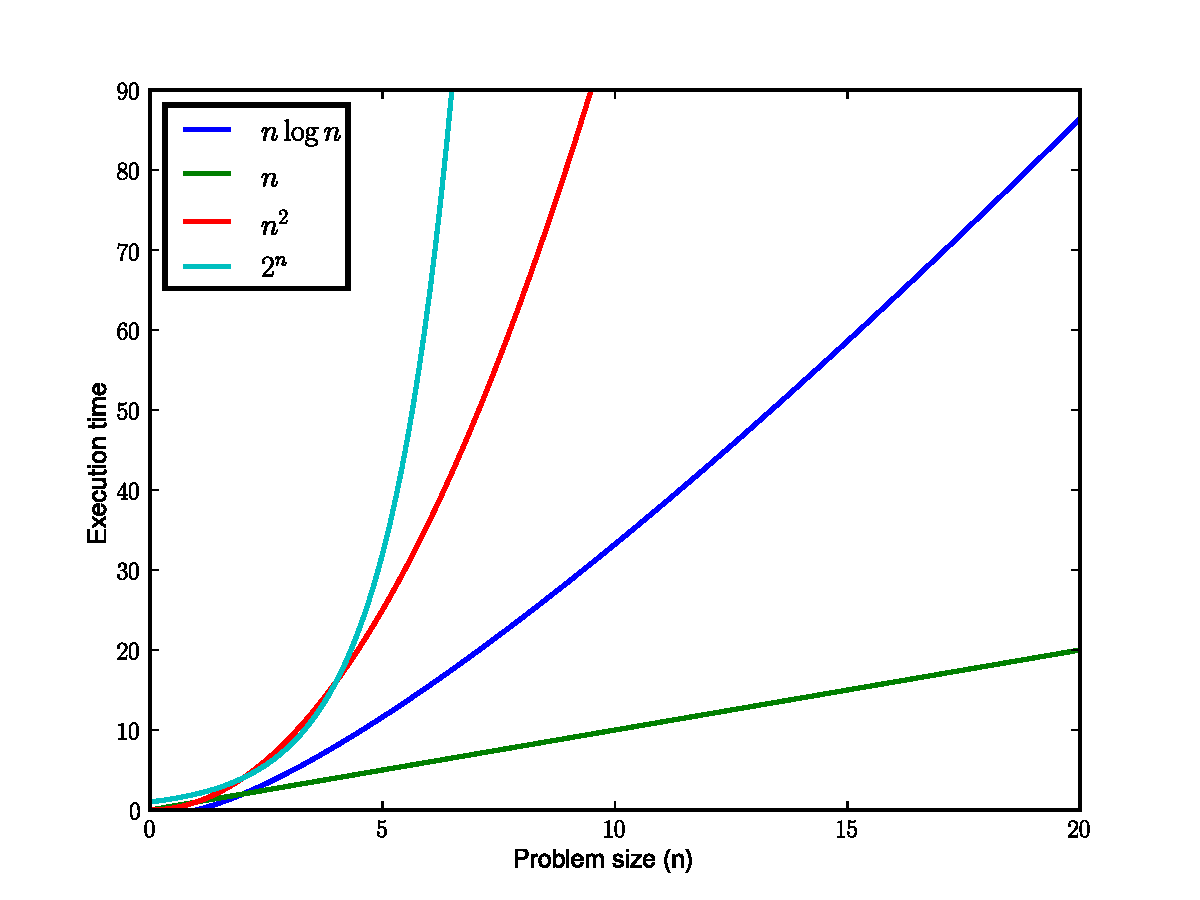
\includegraphics[width=\textwidth]{complexitycurves.pdf}
\caption{Some common asymptotic curves.}
\end{figure}

\begin{definition}[Temporal Complexity]
Let $n$ represent the problem size.  Let $f(n)$ and $g(n)$ be functions mapping natural numbers to positive real numbers. We say that $f \in O(g(n))$ if there exists a real number $c > 0$ and a natural number $n_0$ such that for all natural numbers $n > n_0$, $f(n) \leq cg(n)$.
When this is satisfied, we say that $g(n)$ is an asymptotic upper bound for $f(n)$. 
The notation $f = O(g(n))$ is also common.
\end{definition}

What does this have to do with computer programs?
Every algorithm executed on a computer corresponds to a function
that returns the number of steps taken (and therefore the time)
given an input of size $n$.  Certain problems can be solved with fewer steps,while others require many more.  

For example, given two matrices of size $n$, matrix addition is $O(n^2)$. This is because it takes approximately $n^2$ steps to add $n^2$ elements for our $n \times n$ arrays. 
Comparatively, calculating the inverse of a matrix using Gaussian
row reduction is $O(n^3)$. (There are in fact more efficient
algorithms for matrix inversion.)

How do we determine the temporal complexity of a piece of code?
Calculating the exact temporal complexity of a formula is fairly difficult.
However, to asymptotically analyze a function is fairly straightforward.

\begin{lstlisting}
s = 0
for i in xrange(100):
    s = s + i
\end{lstlisting}

The code above is $O(n)$ because it takes approximately $n$ steps to complete. For-loops are a good indicator of the complexity.  A double for-loop strongly suggests $O(n^2)$ or worse.  Asymptotic analysis reveals that
if we have an array of size $n \times n$ and it takes $x$ seconds to execute an $O(n^2)$ algorithm,
then by increasing the size of the array to $2n \times 2n$, we should expect the same algorithm
to terminate in about $(2)^2 x = 4x$ seconds.  Sometimes, when you don't have code to look at,
you can approximate the asymptotic growth of a function by timing it on various sized inputs.

\begin{problem}
Time the runtime of the following code for \li{n = 1000, 2000, 4000, 8000}.

\lstinputlisting[style=fromfile]{test.py}

Now write a function that takes no arguments and does the following: 
\begin{enumerate}
\item plot the four runtimes (use \li{[1000, 2000, 4000, 8000]} or an equivalent array object as your domain).
The plot should look like Figure \ref{prob1} if using the \li{plt.scatter} command. 
\item return the average ratio between successive runtimes (one such ratio would be the runtime for $n = 2000$ divided by the runtime for $n = 1000$).
\end{enumerate}
\end{problem}

\begin{figure}
\centering
\includegraphics[width=\textwidth]{prob1.pdf}
\caption{The plot of problem 1}
\label{prob1}
\end{figure}

We can also classify an algorithm by the amount of memory it needs to execute.  We will use the term \emph{spatial complexity} to measure the amount of memory an algorithm uses.  The definition of spatial complexity is the same as the definition for temporal complexity with the obvious difference that $n$ refers to space rather than time.
In practice, spatial and temporal complexity are not completely independent of each other. The amount of memory required by an algorithm can affect its speed in several ways. The most important consideration is when the memory usage exceeds the amount of available RAM. When this occurs, the machine must use the hard disk or some other slower storage method. Doing so makes the read and write operations become substantially slower.

\section*{Sparse Matrices}
A sparse matrix is a matrix that has relatively few nonzero elements.
SciPy has several different ways to store sparse matrices. Each way has its own benefits and the reader is encouraged to do additional research. 

\begin{table}
\centering
\begin{tabular}{|l|l|}
\hline
Function & Description \\
\hline
\li{sparse.bsr_matrix()} & Compressed Block Sparse Row\\
\li{sparse.coo_matrix()} & Coordinate\\
\li{sparse.csc_matrix()} & Compressed Sparse Column\\
\li{sparse.csr_matrix()} & Compress Sparse Row\\
\li{sparse.dia_matrix()} & Sparse Diagonal\\
\li{sparse.dok_matrix()} & Dictionary of Keys\\
\li{sparse.lil_matrix()} & Linked List\\
\hline
\end{tabular}
\caption{Sparse matrix representations in SciPy}
\label{smr}
\end{table}

The following showcases some of SciPy's sparse matrix representation functions listed in Table \ref{smr}

\begin{lstlisting}
In [1]: import numpy as np

In [2]: from scipy import sparse

In [3]: A = np.diagflat([2, 3, 4])

In [4]: A
Out[4]: 
array([[2, 0, 0],
       [0, 3, 0],
       [0, 0, 4]])

In [5]: B = sparse.csc_matrix(A)

In [6]: B
Out[6]: 
<3x3 sparse matrix of type '<type 'numpy.int64'>'
	with 3 stored elements in Compressed Sparse Column format>

In [7]: C = B.todense()

In [8]: C
Out[8]: 
matrix([[2, 0, 0],
        [0, 3, 0],
        [0, 0, 4]])

\end{lstlisting}


Notice that the matrix $A$ has only three non-zero entries so we consider it to be a sparse matrix.
In memory, an array stores a piece of data (be it an integer, float, or complex number) in each entry. This means that a $3 \times 3$ matrix requires a total 9 blocks of memory.
However, if we leverage the sparsity of $A$ we realize that we really only need to store 3 numbers.
The \li{sparse} methods do exactly this: they store only the non-zero entries and their locations in the matrix.
An entire array is no longer being stored, decreasing complexity.  

SciPy has many methods for performing operations on sparse matrices. For example, to convert back to a dense matrix we use the \li{todense()} method (of the sparse matrix). We can also convert between the different types of sparse matrices.

Note that if you want to make a sparse diagonal matrix, the best way to do so isn't by creating a diagonal matrix using \li{diagflat()} and then making it sparse by using \li{sparse}. Instead it is much better to use the \li{sparse.spdiags()} method like so:

\begin{lstlisting}
In [1]: # sparse.spdiags(data, diags, m, n)
In [2]: sparse.spdiags([2, 3, 4], 0, 3, 3) 
\end{lstlisting}

Note that \li{diags=0} sets our data along the main diagonal for an $m \times n$ matrix. If \li{diags} $> 0$ then our data is set along the indicated upper diagonal. Similarly, if \li{diags} $< 0$ then our data is set along the indicated lower diagonal. 

Often, when we are using sparse matrices it is because we are dealing with matrices that are otherwise too large to be handled efficiently when represented in full form.

%insert problem here that lets them play around with large sparse matrices in diff forms

\section*{Banded Matrices}
A banded matrix is one whose only non-zero entries are diagonal
strips.  For example, the matrix
\begin{equation*}
A = \begin{pmatrix}
1 & 2 & 0 & 0 \\
3 & 4 & 5 & 0 \\
0 & 6 & 7 & 8 \\
0 & 0 & 9 & 10
\end{pmatrix}
\end{equation*}
is banded because the only non-zero entries are located in three nonzero diagonals.  This particular type of banded matrix is called a tri-diagonal matrix.

Banded matrices are easily created using the \li{diagflat()} method.
For example, the matrix $A$ from above can be created by doing:

\begin{lstlisting}
In [1]: # np.diagflat(data, k=0)
In [2]: np.diagflat([3, 6, 9], -1) + np.diagflat([1, 4, 7, 10], 0) + np.diagflat([2, 5, 8], 1)
Out[2]: 
array([[ 1,  2,  0,  0],
       [ 3,  4,  5,  0],
       [ 0,  6,  7,  8],
       [ 0,  0,  9, 10]])

\end{lstlisting}
Note that \li{data} must be a flattened array and the keyword argument \li{k} is an integer that determines which diagonal is set with the given data. 

However, creating this tri-diagonal required using \li{np.diagflat} three times. Often, a better way to create a tri-diagonal is it use the \li{sparse.spdiags()} method.
This is because many banded matrices are sparse.

For example, we can create the same matrix from above using the command:
\begin{lstlisting}
In [1]: Z = np.array([[3,6,9,0],[1,4,7,10],[0,2,5,8]])
In [2]: sparse.spdiags(Z, [-1, 0, 1], 4, 4)
Out[2]: 
<4x4 sparse matrix of type '<type 'numpy.int64'>'
	with 10 stored elements (3 diagonals) in DIAgonal format>

\end{lstlisting}

For more information, check the documentation by typing \li{sparse.spdiags?}.

\begin{problem}
Write a function that takes an integer argument \li{n} and returns a full $n\times n$
tri-diagonal array with $2$'s along the diagonal and $-1$'s along
the two sub-diagonals above and below the diagonal.
\label{full_tridiag}
\end{problem}

We will now create a tri-diagonal array with uniformly distributed random entries. This example also demonstrates the efficiency of using sparse arrays.

\begin{lstlisting}
In [1]: B = np.random.rand(3, 10000)

In [2]: A = sparse.spdiags(B, range(-1, 2), 10000, 10000)

In [3]: denseA = A.todense() # Only do this if you have lots of memory.

In [4]: A.data.nbytes # About .24MB of memory.
Out[4]: 240000

In [5]: denseA.nbytes # About 762.9MB of memory.
Out[5]: 800000000

\end{lstlisting}

Although the complete matrix is too large to represent in memory,
we can still visualize it using the \li{plt.spy()} command from Matplotlib,
which essentially shows the location of non-zero entries in a matrix.
The output of \li{plt.spy(A)} in this case is shown in Figure \ref{fig:mpl_spy}.

\begin{figure}
\centering
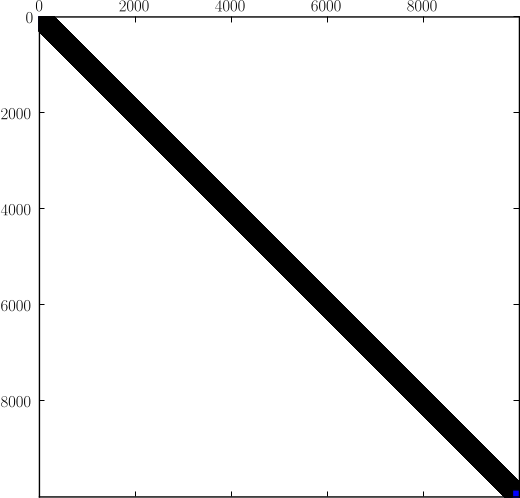
\includegraphics[width=\textwidth]{spy.png}
\caption{The output of the \li{spy()} command}
\label{fig:mpl_spy}
\end{figure}

\begin{problem}
Write a function that accepts an integer argument \li{n} and returns the same array as Problem \ref{full_tridiag}, but as a sparse array.
You must build this as a sparse matrix from the beginning.
Hint: Use the \li{sparse.spdiags()} method with \li{format='csr'}.
\label{prob:sparse_tridiag}
\end{problem}

\section*{Using Sparse Matrices}
Consider the linear system $A x = b$, where $A$ is a $100000\times 100000$ tri-diagonal matrix.
To store a full matrix of that size in your computer, it would normally require 10 billion double-precision floating-point numbers.  Since it takes 8 bytes to store a double, it would take roughly 80GB to store the full matrix.  For most desktop computers, that fact alone makes the system numerically prohibitive to solve.
The temporal complexity of this problem is even more problematic. Methods for directly solving an arbitrary linear system are usually $O(n^3)$. As a result, even if the computer could store an 80GB matrix in RAM, it would still take several weeks to solve the system.  However, since we don't have computers with that much available RAM, most of the
matrix would have to be stored on the hard drive, so the computation would probably take between $6$ months to a year.

The point is that even the next generation of computers will
struggle with solving arbitrary linear systems of this size in a reasonable period of time.  However, if we take advantage of the sparse structure of the tri-diagonal matrix, we can solve the linear system, even with a modest modern computer.  This is because all of those zeros don't need to be stored and we don't need to do as many operations to row reduce the tri-diagonal system.

Let's first compute the spatial complexity of the above system when considered as a sparse matrix.  There are three diagonals that have roughly $100000$ non-zero entries.  That's $300000$
double-precision floating point numbers, which is about 2.4 MB (Less storage than your favorite song).  As a result, it will easily fit into the computer's RAM.  Furthermore, the temporal complexity for solving a tri-diagonal matrix is $O(n)$. Let's see how long it takes to solve the system for random data:

\begin{lstlisting}
In [1]: from scipy.sparse import linalg as sparla
In [2]: D = np.random.rand(3, 100000)
In [3]: b = np.random.rand(1, 100000)
In [4]: A = sparse.spdiags(D,[-1,0,1],100000,100000, format='csr')
In [5]: def solSys():
   ....:     return sparla.spsolve(A, b)
   ....: 

In [6]: timeit solSys()

\end{lstlisting}


\begin{problem}
Write a function that accepts an integer argument \li{n} as well as a keyword argument \li{sparse} whose value is either \li{True} or \li{False} (default to \li{False}). Then do the following:
\begin{enumerate}
\item Inside of the function, use your previous solutions to generate an $n \times n$ tri-diagonal array $A$ -- either sparse or full depending on the value of the \li{sparse} argument.
\item Generate an $n \times 1$ random array $b$
\item Solve the system $Ax = b$, using either \li{scipy.sparse.linalg.spsolve} or \li{scipy.linalg.solve}
(again depending on the value of \li{sparse}) and return the solution.
\item Time the function for \li{n = 2000} using both the sparse and the full option.
\end{enumerate}
\end{problem}

\begin{problem}
Write a function that accepts an integer argument \li{n} and returns $\lambda n^2$, where
$\lambda$ is the smallest eigenvalue of the same $n \times n$ sparse tri-diagonal array as described above.

To calculate $\lambda$, use \li{scipy.sparse.linalg.eigs}. You will need to set the \li{which = 'SM'}
optional argument. Further, if \li{A} is your tri-diagonal sparse matrix, you will need to use
\li{A.asfptype()} as the argument for the \li{eigs} function (so that the matrix has the right data type).
Check the documentation of the \li{eigs} function to see what it returns, so that you will know how to
get the smallest eigenvalue.

What value does $\lambda n^2$ approach as $n \rightarrow \infty$?
Hint: It's the square of an important number.
This is related to operator theory: the second derivative operator has this eigenvalue in certain cases.
\end{problem}

\section*{Other Sparse Commands}
One important method of sparse matrix objects is the \li{nonzero()} method, which is related to the number of nonzero entries in the matrix. This number is important because it is an indicator of the amount of time and space that is required to operate on the sparse matrix.
You should be aware that there is some overhead to using and storing the sparse matrix data structure. Sparsely represented matrices are very beneficial when the number of nonzero entries is relatively small compared to the total number of entries.
When the matrix has many nonzero entries, a sparse representation becomes disadvantageous.
To see this, observe: 

\begin{lstlisting}
In [1]: A = np.random.rand(600, 600)

In [2]: B = sparse.csc_matrix(A)

In [3]: def square(A):
   ....:     return np.power(A, 2)
   ....: 

In [4]: timeit square(A)
100 loops, best of 3: 9.53 ms per loop

In [5]: timeit square(B)
1 loops, best of 3: 941 ms per loop
\end{lstlisting}

Notice that it takes much longer to square the sparse matrix.
This is because the sparse matrix data structure is optimized for matrices that are actually sparse. The array $A$ is entirely nonzero. Thus, you incur the overhead of the sparse array representation without any benefits since there are no entries you are not required to store or compute.

To summarize, only use a sparse matrix when your matrix is in fact sparse. Using sparse matrices for mostly nonzero arrays will negatively impact performance and memory requirements.

Just as with dense arrays, we can pre-allocate sparse matrices.
Sometimes it is necessary to create sparse matrices that do not have a nice banded pattern. We initialize a sparse matrix just like any other array. The most efficient sparse matrix for pre-allocation is \li{LIL}. Once you are done constructing the sparse matrix and wish to perform calculations, you should convert to a more efficient sparse matrix (CSR or CSC).


\begin{lstlisting}
In [1]: Z = sparse.lil_matrix((400, 300))

In [2]: Z[1,34] = 23

In [3]: Z[23,32] = 56

In [4]: Z[2,:] = 13.2

In [5]: Z
Out[5]: 
<400x300 sparse matrix of type '<type 'numpy.float64'>'
	with 302 stored elements in LInked List format>

\end{lstlisting}

When the matrix \li{Z} from above is initialized, all entries of the $400 \times 300$ \li{LIL} sparse matrix are assumed to be zero. 
We can then work with the sparse matrix as though it were a dense array.
Note that only 302 elements are being stored for a matrix with 120000 possible entries. 
 
